% !TEX root = paper.tex
% !TEX encoding = UTF-8 Unicode





% !TEX root = paper.tex
% !TEX encoding = UTF-8 Unicode

\begin{figure}
\begin{subfigure}[b]{\linewidth}
\begin{center}
\caption{Russian-English}
\label{fig:mean_adequacy_score_ru}
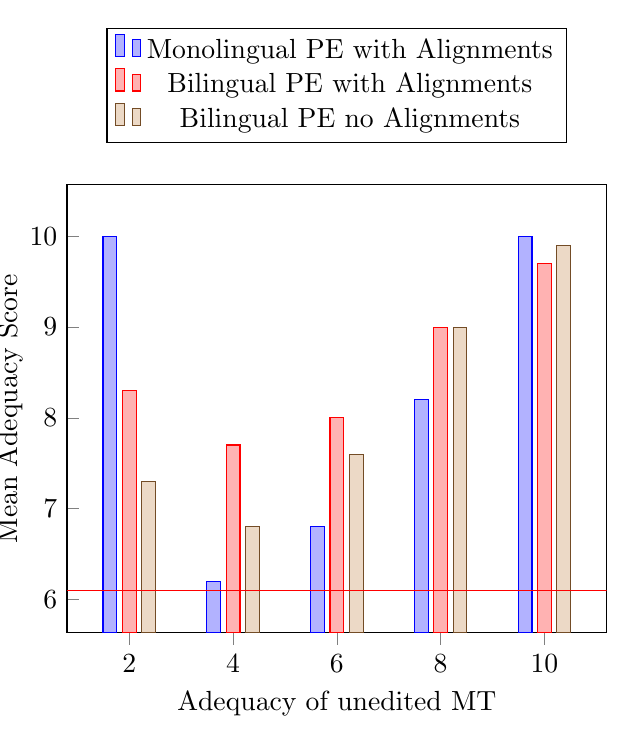
\begin{tikzpicture}[trim left={(-0.5,0)}]
\begin{axis}[
	%at={(10,0)},
	x tick label style={
		/pgf/number format/1000 sep=},
	ylabel shift={-0.15cm},
	ylabel=Mean Adequacy Score,
	enlargelimits=0.15,
	xtick pos=left,
	ytick pos=left,
	xlabel={Adequacy of unedited MT},
	%,
%	legend style={at={(0.5,-0.15)}},
%		anchor=north,legend columns=-1},
	legend style={at={(0.5,1.35)},anchor=north},
	ybar,
	bar width=5pt,
]
\addplot 
	coordinates {(2,10.0) (4,6.2)
		 (6,6.8) (8,8.2) (10,10)};

\addplot 
	coordinates {(2,8.3) (4,7.7)
		 (6,8.0) (8,9.0) (10,9.7)};

\addplot 
	coordinates {(2,7.3) (4,6.8)
		 (6,7.6) (8,9.0) (10,9.9)};

\addplot[red,sharp plot,update limits=false] 
	coordinates {(-1,6.1) (12,6.1)};

\legend{Monolingual PE with Alignments,Bilingual PE with Alignments,Bilingual PE no Alignments}
\end{axis}
\end{tikzpicture}
\end{center}
\end{subfigure}
\ \\
\begin{subfigure}[b]{\linewidth}
\begin{center}
\caption{Spanish-English}
\label{fig:mean_adequacy_score_es}
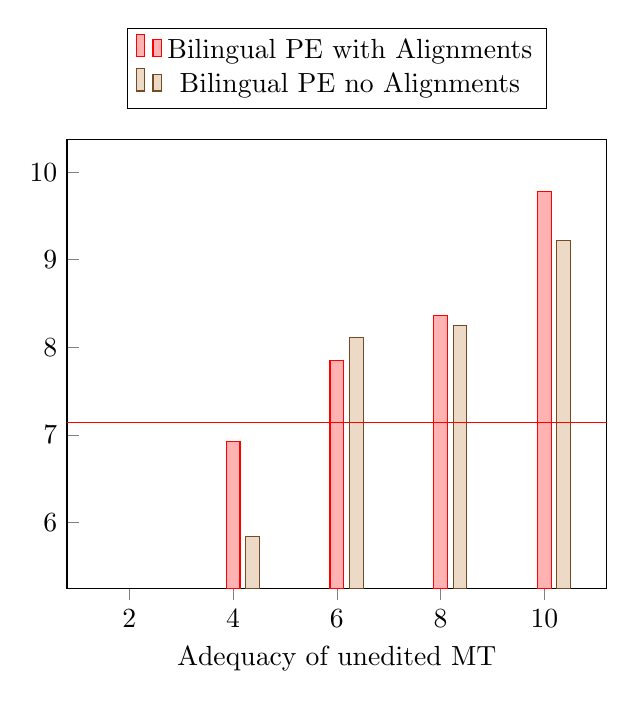
\begin{tikzpicture}[trim left={(-0.5,0)}]
\begin{axis}[
	%at={(10,0)},
	x tick label style={
		/pgf/number format/1000 sep=},
	ylabel shift={-0.15cm},
%	ylabel=Mean Adequacy Score,
	enlargelimits=0.15,
	xtick pos=left,
	ytick pos=left,
	xlabel={Adequacy of unedited MT},
	legend style={at={(0.5,1.25)},anchor=north},
	ybar,
	xmin=2,
	bar width=5pt,
]
\addplot 
	coordinates {};

%	Adequacy with align	Adequacy w/o align
%2		
%4	6.92	5.84
%6	7.85	8.11
%8	8.36	8.25
%10	9.78	9.22

\addplot coordinates {(4,6.92) (6,7.85) (8,8.36) (10,9.78) };
\addplot coordinates {(4,5.84) (6,8.11) (8,8.25) (10,9.22) };
\addplot[red,sharp plot,update limits=false] coordinates { (-1,7.14) (12,7.14) };
	
%\addplot coordinates {(4,6.6) (6,7.7272727272727275) (8,8.818181818181818) (10,9.923076923076923) };
%\addplot coordinates {(4,6.0) (6,8.090909090909092) (8,8.909090909090908) (10,9.384615384615385) };
%\addplot[red,sharp plot,update limits=false] coordinates { (-1,7.686274509803922) (12,7.686274509803922) };

\legend{Bilingual PE with Alignments,Bilingual PE no Alignments}
\end{axis}
\end{tikzpicture}
\end{center}
\end{subfigure}
\caption{Mean adequacy score, categorized by the adequacy score of the unedited MT. The red horizontal line indicates the mean adequacy score (Russian-English: 6.1; Spanish-English: 7.1) of the unedited MT.}
\label{fig:mean_adequacy_score}
\end{figure}



\section{Results}
\label{sec:results}


\subsection{Rating Translation Adequacy}

Following the methodology outlined in \S\ref{sec:translation_quality}, all post-edited output as well as all machine translations were evaluated by bilingual human judges using the adequacy scales shown in Table~\ref{judge_guidelines} \vpageref{judge_guidelines}.


\subsubsection{Rating Adequacy of Russian-English}

%\subsection{Rating of translations}

Following the adequacy guidelines from \S\ref{sec:translation_quality}, %shown in Table~\ref{judge_guidelines_russian},
%
an experienced English-Russian translator and grader rated all English output translations of the Russian-English post-edited segments.
%
In addition, all English machine translations of the Russian documents were manually rated for adequacy.
% as well as the machine translation segments.
%in both human-readable tabular form and machine-readable CSV form in the attached dataset supplement.}

For each segment, the human rater was presented with a vertically-arranged list showing all variants of that segment.
%
The first entry in each list was the segment in the source language (Russian).
%
The source segment was followed by the reference translation in English.
%
The subsequent eight entries were English translations of the source segment, presented in a randomized order.
%
The English translations included the unedited machine translation output, as produced by Moses,
%
a post-edited translation produced by a monolingual post-editor from \citet{2014_WMT_Schwartz_etal},
%
and the six post-edited translations produced by the Russian-English bilingual post-editors in this study.

All Russian-English translations were rated using the translation adequacy scale in Table \Vref{judge_guidelines_russian}, with possible ratings ranging from  2 (translation makes no sense) to 12 (translation is superior to the reference translation).

%The human rater was presented with blocks of 10 lines arranged in a vertical list:
%%
%the first line was a source segment, 
%%
%the second was its reference translation, and 
%%
%below these were eight translations for the segment 
%%
%(the machine translation, one monolingual post-edited translation from \citet{2014_WMT_Schwartz_etal}, and six bilingual post-edited translations) 
%%
%listed in random order. 
%%
%The rater was asked to classify all the segment translations on an adequacy scale (see Table \Vref{judge_guidelines_russian}) ranging from 2 (translation makes no sense) to 12 (translation is superior to the reference translation). 



\subsubsection{Rating Adequacy of Spanish-English}

Following the adequacy guidelines from \S\ref{sec:translation_quality}, 
%
an experienced Spanish-English translator and grader worked in cooperation with a second Spanish-English bilingual to rate all English output translations of the Spanish-English post-edited segments.
%
In addition, all English machine translations of the Spanish documents were manually rated for adequacy.
%
%One experienced Spanish-English translator and grader and one Spanish-English bilingual rated all post-edited segments as well as the MT segments.
%%
%They did this in cooperation.
For each segment, the human raters were presented with a vertically-arranged list showing all variants of that segment.
%
The first entry in each list was the segment in the source language (Spanish).
%
The source segment was followed by the reference translation in English.
%
The subsequent five entries were English translations of the source segment, presented in a randomized order.
%
The English translations included the unedited machine translation output, as produced by Bing Translator,
%
and the four post-edited translations produced by the Spanish-English bilingual post-editors in this study.

Unlike the Russian documents, no reference translation was available for the Spanish documents; for this reason (as described in \S\ref{sec:translation_quality}), the top category (12) used in evaluating Russian-English segments was omitted from the Spanish-English evaluation.
%
All Spanish-English translations were rated using the translation adequacy scale in Table \Vref{judge_guidelines_spanish}, with possible ratings ranging from  2 (translation makes no sense) to 10 (the meaning of the Spanish sentence is fully conveyed in the English translation).
%
%
%%
%The raters were presented with blocks of six lines arranged in a vertical list: the first line was a source segment, the second was its machine translation, and below these were four translations for the segment listed in random order.
%%
%The raters were asked to classify all the segment translations on an adequacy scale (see Table \Vref{judge_guidelines_spanish}) ranging from 2 (translation makes no sense) to 10 (the meaning of the Spanish sentence is fully conveyed in the English translation). 
% 
%For the rating of the segments in this experiment the top category used for the evaluation of the Russian segments was removed because in the Spanish experiment we did not use a reference translation.



\subsection{Adequacy Results}

Figure~\ref{fig:percentage_segments} \vpageref[above]{fig:percentage_segments} presents the percentage of segments judged to be in each adequacy category.
%
Mean adequacy scores for each experimental condition are presented in Figure~\ref{fig:mean_adequacy_score} \vpageref[above]{fig:mean_adequacy_score}.
%
By subtracting the adequacy score of each machine translated segment, we obtain the adequacy gain obtained by post-editing;
%
these values are presented in Figure~\ref{fig:mean_adequacy_gain} \vpageref[above]{fig:mean_adequacy_gain}.
%The above effect can be seen clearly in Figure \Vref{fig:mean_adequacy_gain}, where we show mean gain in adequacy over unedited MT
%
%We also calculate the adequacy improvements of post-edited translations over unedited machine translations; such mean gains in adequacy are presented in Figure~\ref{fig:mean_adequacy_gain} \vpageref[above]{fig:mean_adequacy_gain}.
%
Finally, Figure~\ref{fig:mean_adequacy_score_per_posteditor} \vpageref[above]{fig:mean_adequacy_score_per_posteditor} presents mean adequacy score by post-editor.
%
We now analyze these results by experimental condition.

\subsubsection{Machine Translation Adequacy}

In Figure~\ref{fig:percentage_segments} \vpageref[above]{fig:percentage_segments}, we observe that the Russian-English machine translation segments tend to be of lower quality (as measured by adequacy), while the Spanish-English machine translation segments tend to be of higher quality.
%
Two-thirds of Russian-English machine translation segments are judged to have major errors (ratings 2-6), while one-third are rated as mostly or completely correct (8-12).
%
Contrast this with the Spanish-English machine translations segments; 
%
less than one-third are judged to have major errors (ratings 2-6), while the majority (over two-thirds) are rated as mostly or completely correct (8-10).


% !TEX root = paper.tex
% !TEX encoding = UTF-8 Unicode

\begin{figure}
\begin{subfigure}[b]{\linewidth}
\begin{center}
\caption{Russian-English}
\label{fig:mean_adequacy_gain_ru}
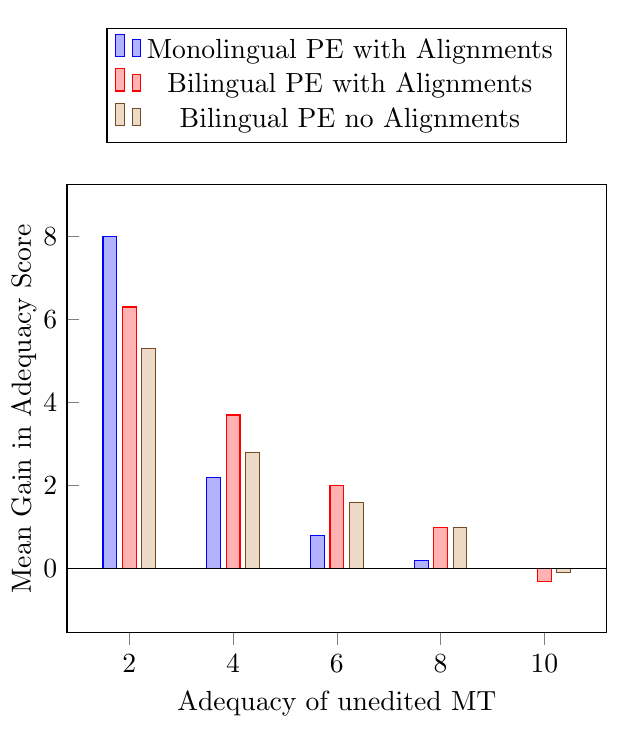
\begin{tikzpicture}[trim left={(-0.5,0)},trim axis right]
\begin{axis}[
	x tick label style={
		/pgf/number format/1000 sep=},
	ylabel shift={-0.15cm},
	ylabel=Mean Gain in Adequacy Score,
	xlabel={Adequacy of unedited MT},
%	ymin={0.1},
	enlargelimits=0.15,
	legend style={at={(0.5,1.35)},anchor=north},
	ybar,
	bar width=5pt,
	xtick pos=left,
	ytick pos=left,
%	ymin=0.0,
]
\addplot 
	coordinates {(2,8.0) (4,2.2)
		 (6,0.8) (8,0.2) (10,0)};

\addplot 
	coordinates {(2,6.3) (4,3.7)
		 (6,2.0) (8,1.0) (10,-0.3)};

\addplot 
	coordinates {(2,5.3) (4,2.8)
		 (6,1.6) (8,1.0) (10,-0.1)};

\addplot[black,sharp plot,update limits=false] 
	coordinates {(-1,0) (12,0)};

\legend{Monolingual PE with Alignments,Bilingual PE with Alignments,Bilingual PE no Alignments}
\end{axis}
\end{tikzpicture}
\end{center}
\end{subfigure}
\ \\ \ \\
\begin{subfigure}[b]{\linewidth}
\begin{center}
\caption{Spanish-English}
\label{fig:mean_adequacy_gain_es}
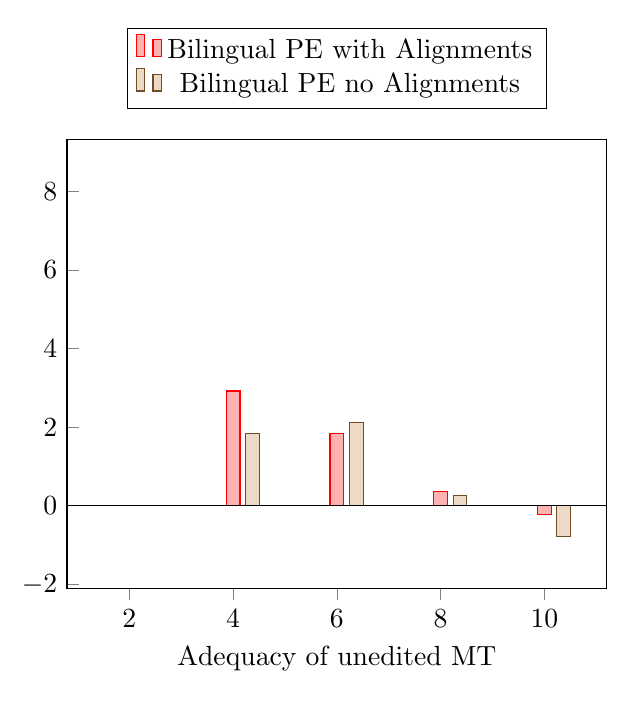
\begin{tikzpicture}[trim left={(-0.5,0)},trim axis right]
\begin{axis}[
	x tick label style={
		/pgf/number format/1000 sep=},
	ylabel shift={-0.15cm},
%	ylabel=Mean Gain in Adequacy Score,
	xlabel={Adequacy of unedited MT},
%	ymin={0.1},
	enlargelimits=0.15,
	legend style={at={(0.5,1.25)},anchor=north},
	ybar,
	bar width=5pt,
	xtick pos=left,
	xmin=2,
	ytick pos=left,
	ymax = 8,
%	ymin=0.0,
]
\addplot 
	coordinates {};

%	Gain with align	Gain w/o align
%2		
%4	2.92	1.84
%6	1.85	2.11
%8	0.36	0.25
%10	-0.22	-0.78

\addplot coordinates {(4,2.92) (6,1.85) (8,0.36) (10,-0.22) };
\addplot coordinates {(4,1.84) (6,2.11) (8,0.25) (10,-0.78) };

%\addplot coordinates {(4,2.6) (6,1.7272727272727273) (8,0.8181818181818182) (10,-0.07692307692307693) };
%\addplot coordinates {(4,2.0) (6,2.090909090909091) (8,0.9090909090909091) (10,-0.6153846153846154) };

\addplot[black,sharp plot,update limits=false] 
	coordinates {(-1,0) (12,0)};

\legend{Bilingual PE with Alignments,Bilingual PE no Alignments}
\end{axis}
\end{tikzpicture}
\end{center}
\end{subfigure}
\caption{Mean gain in adequacy score over unedited MT, categorized by the adequacy score of the unedited MT.}
\label{fig:mean_adequacy_gain}
\end{figure}


\subsubsection{Russian-English Adequacy}

%The post-edited English segments

The mean adequacy score when bilingual participants were presented with alignments was 8.35.
%
When alignments were omitted from the post-editing tool, the mean adequacy score was 7.85.  
%
A Wilcoxon signed-rank test \citep{1945_Wilcoxon} showed that when participants were presented with alignments the ratings of their translations were significantly higher than when participants post-edited without access to alignments (N = 6, Z = -2.207, p = 0.027).



\subsubsection{Spanish-English Adequacy}

The mean adequacy score when Spanish bilingual participants were presented with alignments was 8.65. When alignments were omitted from the post-editing tool, the mean adequacy score was 8.57. These means are not significantly different.



%Our results suggest that when machine translation quality is low, bilingual post-editors may produce higher quality translations when presented with bilingual alignment links between source words and machine-translated target words.
%
%In addition to rating each post-edited translation, our bilingual human judge rated the adequacy of the unedited MT segments.
%%
%We thereby obtained direct human judgements of MT quality.
%%
%Because we care about the adequacy of post-edited translations, we consider actual human judgements to be preferable to automated metrics such as BLEU \citep{2002_ACL_Papineni_etal}, which at best serve as a flawed proxy for human judgements.

%We partition the data according to the MT quality as measured by our human judge in terms of adequacy.
%%
%For each partition, we then calculate the mean adequacy score of post-edited segments, once for the case where post-editors were presented with alignment data, and once for the case where alignments were not presented.
%%
%In addition, we perform the same average calculation for the monolingual post-edited segments of Docs A and B from \citet{2014_WMT_Schwartz_etal}.
%%
%The results are shown in Figure \ref{fig:mean_adequacy_score}.


%\clearpage 


% !TEX root = paper.tex
% !TEX encoding = UTF-8 Unicode

\begin{figure*}[t]
\begin{subfigure}[b]{.5\linewidth}
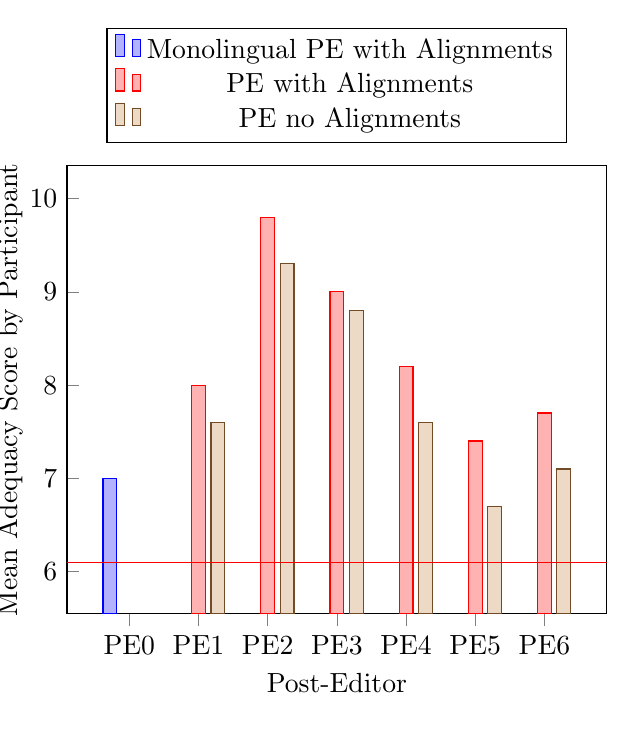
\begin{tikzpicture}[trim left={(-0.5,0)},trim axis right]
\begin{axis}[
    ybar,
    enlargelimits=0.15,
    legend style={at={(0.5,1.05)},anchor=south},
   ylabel={Mean Adequacy Score by Participant},
   xlabel={Post-Editor},
   % symbolic x coords={PE0,PE1,PE2,PE3,PE4,PE5,PE6},
    xtick={0,1,2,3,4,5,6},
    xticklabels={PE0,PE1,PE2,PE3,PE4,PE5,PE6},
	xtick pos=left,
	ytick pos=left,
	ylabel shift={-0.15cm},
    %xtick=data,
    %nodes near coords,
    %nodes near coords align={vertical},
    bar width=5pt
    ]

\addplot coordinates { (0,7.0) (0,6.1)};
\addplot coordinates { (1,8.0) (2,9.8) (3,9.0) (4,8.2) (5,7.4) (6,7.7)};
\addplot coordinates { (1,7.6) (2,9.3) (3,8.8) (4,7.6) (5,6.7) (6,7.1)};

\addplot[red,sharp plot,update limits=false] 
	coordinates {(-1,6.1) (8,6.1)};
	%node[above] at (axis cs:3,6.1) {Unedited MT};
	
%%\addplot coordinates {(tool8,1) (tool9,1) (tool10,1)};
\legend{Monolingual PE with Alignments, PE with Alignments,PE no Alignments}
\end{axis}
\end{tikzpicture}
\caption{Russian-English}
\label{fig:mean_adequacy_score_per_posteditor_ru}
\end{subfigure}
\begin{subfigure}[b]{.5\linewidth}
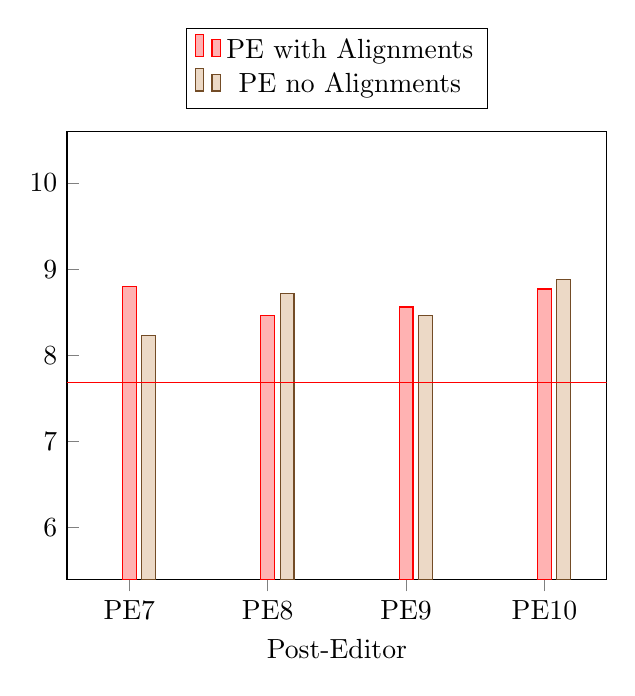
\begin{tikzpicture}[trim left={(-0.5,0)},trim axis right]
\begin{axis}[
    ybar,
    enlargelimits=0.15,
    legend style={at={(0.5,1.05)},anchor=south},
%   ylabel={Mean Adequacy Score by Participant},
   xlabel={Post-Editor},
   % symbolic x coords={PE0,PE1,PE2,PE3,PE4,PE5,PE6},
    xtick={1,2,3,4},
    xticklabels={PE7,PE8,PE9,PE10},
	xtick pos=left,
	ytick pos=left,
	ylabel shift={-0.15cm},
	ymin=6,
	ymax=10,
    %xtick=data,
    %nodes near coords,
    %nodes near coords align={vertical},
    bar width=5pt
    ]

\addplot coordinates {};
\addplot coordinates {(1,8.8) (2,8.461538461538462) (3,8.56) (4,8.76923076923077) };
\addplot coordinates {(1,8.23076923076923) (2,8.72) (3,8.461538461538462) (4,8.88) };
\addplot[red,sharp plot,update limits=false] coordinates { (-1,7.686274509803922) (12,7.686274509803922) };

%%\addplot coordinates {(tool8,1) (tool9,1) (tool10,1)};
\legend{PE with Alignments,PE no Alignments}
\end{axis}
\end{tikzpicture}
\caption{Spanish-English}
\label{fig:mean_adequacy_score_per_posteditor_es}
\end{subfigure}
\caption{Mean adequacy score per post-editor. The red horizontal line indicates the mean adequacy score (Russian-English: 6.1; Spanish-English: 7.7) of the unedited MT.}
\label{fig:mean_adequacy_score_per_posteditor}
\end{figure*}


\subsection{Timing Results}

\subsubsection{Russian-English Timing}

The times taken by the Russian-English post-editors to post-edit each text were recorded manually to the nearest minute. The mean times were 33 minutes for texts with alignment and 40 minutes for texts without alignment. This difference approached significance (p = .082).

\subsubsection{Spanish-English Timing}

The times taken by the Spanish-English post-editors to post-edit each text were recorded by the keylogger to nearest millisecond. The mean times were 16.36 minutes for texts with alignment and 16.66 minutes for texts without alignment. This difference was not statistically significant.
%
The shorter editing times for Spanish-English may in part be explained by the shorter length of these documents.


\section{Analysis and Related Work}
\label{sec:background}

Our results suggest that when machine translation quality is poor (2--4), bilingual post-editors may produce higher quality translations when presented with bilingual alignment links between source words and machine-translated target words.
%
Alternatively, when machine translation quality is high (8--12), no effect is seen by presenting alignment visualizations.
%
We explain this by hypothesizing that word alignment visualization may enable post-editors to better recover from certain types of translation errors produced by MT systems; when MT quality is high enough that such errors are absent, word alignment visualization may no longer play a restorative role.


%
%
%We observe that when MT quality was poor (adequacy categories 2--6), bilingual post-editors consistently produced higher quality post-edited translations when alignments were shown.
%
%On the other hand, when MT quality is high (adequacy categories 8--10), little or no impact to adequacy quality was observed when alignments were shown. 
%%
%By subtracting the adequacy score of each machine translated segment, we obtain the adequacy gain obtained by post-editing.
%%
%The above effect can be seen clearly in Figure \Vref{fig:mean_adequacy_gain}, where we show mean gain in adequacy over unedited MT;
%%
%post-editing makes the most difference when MT quality is poor, and in those cases the presence of alignment links improves post-editing as measured by adequacy.


We examine the effect that alignment link visualization has on each bilingual post-editor in Figure \ref{fig:mean_adequacy_score_per_posteditor} \vpageref[above]{fig:mean_adequacy_score_per_posteditor}.
%
In the Russian-English condition, where overall MT quality is poor, we observe that post-editing quality varies widely between post-editors (with PE2 and PE3 performing best).
%
For all six bilingual post-editors, we observe higher mean adequacy scores when alignment links were presented than when they were omitted from the post-editing tool.
%
We also note that when alignment links were absent, one bilingual post-editor (PE5) performed worse than the monolingual post-editor (PE0) from \citet{2014_WMT_Schwartz_etal}.
%
On the other hand, in the Spanish-English condition, where overall MT quality is good, we observe relatively little variation in quality between the four post-editors.
%
When compared to the unedited machine translations, post-editing resulted in improved mean adequacy for all post-editors, both bilingual and monolingual.

Our results also suggest that post-editing time tends to be reduced for texts with alignment. 
%
These numerical reductions were consistent across all the Russian-English participants with the exception of PE3, but they were not consistent for the Spanish-English participants. 

We hypothesize that texts with alignment are less cognitively demanding to process, and so less effortful to post-edit than texts without alignment. 
%
If this is the case, shorter post-editing times for texts with alignment are consistent with previous findings by \citet{2012_AMTA_Koponen_etal}, who found that per word post-editing times were shorter for segments that were less cognitively demanding because of the linguistic structure. 
%
Related work on cognitive effort in post-editing \citep{2014_AMTA_Lacruz_etal,2014_Lacruz_Shreve} has also shown decreased densities of short pauses when less cognitively demanding segments are post-edited. 



%Finally, in Figure \ref{fig:percentage_segments} we present histograms graphing the percentage of segments in each adequacy category.
%%
%We observe that the majority of unedited machine translations are of relatively poor quality, falling mostly into categories 4 and 6. %, and a few scoring as 12.
%%
%%The monolingual post-editor from \citet{2014_WMT_Schwartz_etal} was able to skew the quality histogram somewhat to the right, with most segments scored as 6 or 10, and a few scored as better than the reference (12).
%The monolingual post-editor improved MT quality somewhat, with most segments scoring as 6 or 10.
%%
%The histogram for bilingual post-editors using no alignments skewed further to the right, peaking at 8.
%%
%The histogram for bilingual post-editors with access to alignments skews farthest to the right, peaking at 10.



